%%& --output-directory=../../pdf/

\documentclass{beamer}
\usepackage[frenchb]{babel}
\usepackage[T1]{fontenc}
\usepackage[utf8]{inputenc}
\usetheme{CambridgeUS}
\usepackage{tikz}
\usepackage{listings}
\usepackage{verbatim}
\usepackage{hyperref}
\usepackage{ulem}
\usepackage{graphicx}

\usetikzlibrary{arrows,shapes}
\lstset { %
	language=bash,
	backgroundcolor=\color{black!5}, % set backgroundcolor
	basicstyle=\footnotesize,% basic font setting
}

\title{IN104 - Solveur de Sudoku - TP3}
\author{Ugo Vollhardt}
\institute{CEA LIST}

\begin{document}
	\maketitle
	\section{Planning}
\begin{frame}
	Déroulement prévisionnel : 
	\setbeamertemplate{enumerate items}[default]
	\begin{enumerate}
		\item Rappels sur Git, mise en place versionnement, structure donnée et premières fonctions de mises à jours de possibilités.
		\item Rappels/introduction à la notion de récursivité, poursuite du travail de la première séance et mise en place des premiers algo de résolution.
		\item Fin d'implémentation des permiers algo de résolution + rappels sur sujet au choix.
		\item Introduction à la librairie GTK+ pour Python et C, implémentation d'une interface minimale.
		\item Séance en autonomie.
		\item Revu des points précédents et approfondissement si besoin.
	\end{enumerate}
	\end{frame}
	
	\section{Amélioration des discrimination des possibilités}
	\begin{frame}
	\frametitle{Amélioration des discrimination des possibilités}
		\begin{itemize}
			\item Méthode par exclusion : Pour une section donnée (Colonne, Ligne ou carré), si une possibilité n'est présente que sur une seule case (même si cette case en a d'autre), alors la valeur de cette case est cette possibilité.
			\item Méthode par n-uplet exclusive :  Pour une section donnée, si n cases contiennent exactement les même n possibilité, alors ces n possibilités peuvent être retirées des possibilités de toutes les autres cases.
			
		\end{itemize}
	\end{frame}

	\begin{frame}
		\frametitle{Interface graphique minimal}
		\begin{columns}[c]
			\begin{column}{5cm}
				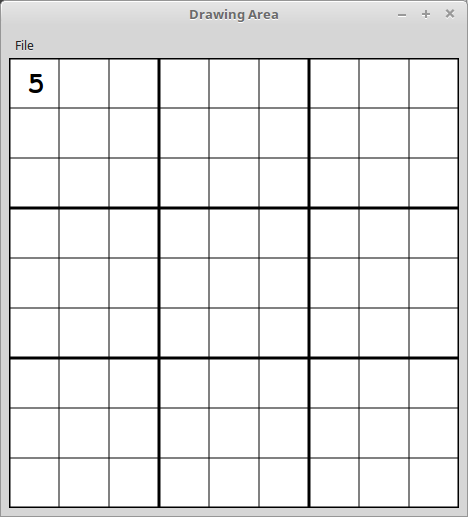
\includegraphics[width=\textwidth,height=\textheight,keepaspectratio]{GUI.png}
			\end{column}
			\begin{column}{7cm}
				Exemples de codes sur le GitHub dans le dossier examples/ \\
				\begin{itemize}
					\item Canvas/ : exemple de l'utilisation de l'objet canvas pour TKinter et Drawing area pour Gtk+. Support pour dessiner.
					\item menu\_bar/ : exemple d'utilisation des classes/types permettant de faire un menu
				\end{itemize}
			\end{column}
		\end{columns}
	\end{frame}

	\section{Objectifs}
	\begin{frame}
	\frametitle{Objectifs de la séance}
	\setbeamertemplate{enumerate items}[default]
	\begin{enumerate}
		\item Finir les implémentations simple et avec forçage.
		\item Ajouter d'autres algorithmes de discrimination pour réduire le recours au forçage.
		\item Designer une interface graphique minimale (affichage grille, petit menu ou boutons).
	\end{enumerate}
	\end{frame}

\end{document}